SysML offers a modeling constructs to represent text-based requirements and
relationship with other modeling elements. The requirements in EA diagram may be
described in a graphical or tree structured format. The requirement may also
appear directly other diagram. The diagram requirements  intent to  may be imported and
exported from other tools in csv or XMI format.

In this particular experiment, a table document has been made in csv format from
the SRS.
Each requirement is represented as a number that corresponds to the numbers and bullet points
of the specification document. From this list of requirements, one can directly
find the corresponding paragraph in the documents. We had also added the
complete text in a text attribute  for helping the reader. 



The requirement list is then automatically translate to a requirement package  in SysML where
each requirement is a \emph{requirement} SysML element. Our requirement contains
the following attributes :
\begin{itemize}
\item ID : the corresponding name from the SRS
\item Body: the corresponding text from the SRS
\end{itemize}
Figure \ref{fig:req-example} shows an example of the requirement representation.
\begin{figure}[htbp]
\centering
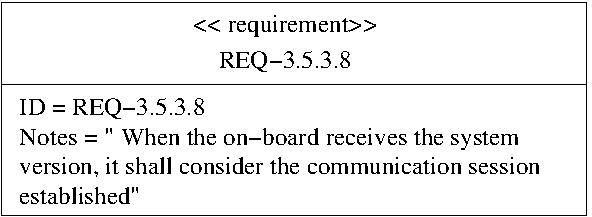
\includegraphics[width=.5\textwidth]{req-example}
\caption{\label{fig:req-example} Example of modeling a requirement}
\end{figure}


Most of requirement refers to the behaviors model as transition of the state-chart
representation.  The link has been made such that each transition satisfy at
least one requirement. Note that in EA, it is not possible to directly link a
transition element to a requirement element, a invariant constraint true has been
added on the transition to make the link.

Others requirement may describe a set of transitions or a more general behavior
property.
In these cases the requirement may be translated as one or more constraints that must be
satisfied by the model. In our model, constraints are invariants expressed in
LTL\cite{PnueliLTL1977}.
SysML does not imposed any language, one can choose other constraints language
such as OCL \cite{ocl2012}.
The following example shows the translation of two requirements into a LTL
properties. The reader should refer to section \ref{sec:deta-model-descr}
for variables and values details.
\begin{description}
\item[REQ-3.5.3.1] "It shall be possible for ERTMS/ETCS on-board equipment and RBC to
initiate a communication session".
\vspace{-1em}
\begin{verbatim}
Finally ((orderOnBoard == 1 || MessageIn == INIT:_SESSION_ORDER || 
MessageIn == INIT_SESSION_TRACK  ) && 
Finally (MessageOut == SESSION_ESTABLISHED))
\end{verbatim}
\end{description}
\begin{description}
\item[REQ-3.5.3.10] "If the establishment of a communication session is
initiated by the RBC, it shall be performed according to the following steps
..."
\vspace{-1em}
\begin{verbatim}
Finally (MessageIn == INIT_SESSION_TRACK && setUp == 1 -> 
Next (MessageOut == SESSION_ESTABLISHED && radioComSession == 1ESTABLISHED)
\end{verbatim}
\end{description}


The requirement diagram only represent the "satisfy" relations between the
requirements and the model. One could refine this diagram and add derive
dependency or containment relationship. Note that in practice we could show the
"satisfy" relations directly on the state-chart view. The separate representation
is more readable. 
